\documentclass[11pt]{article}
\usepackage [russian,english]{babel}
\usepackage [utf8]{inputenc}
\usepackage [T2A]{fontenc}
\usepackage {multicol}
\usepackage {indentfirst}
\usepackage[unicode, bookmarks=true]{hyperref}
\usepackage[pdftex]{graphicx}

\title{\textbf{ARM Trustzone}}
\author{Николай Голиков\\
		<decaprox@gmai.com>}
\date{}
\begin{document}

\maketitle

% % % % % % % % % % % % % % % % % % % % % % % % % % % % % % % % % % % % % % % % % 
\section{Предисловие}
Данная статья является кратким описанием различных аспектов работы с технологией
 Trustzone. И предназначена для содействия быстрому старту в этой области.

Все нижеизложенное основывается на знаниях полученных при работе с платформой
Freescale i.MX53, но частично может быть актуально и для других платформ имеющих
поддержку данной технологии.

На данный момент эта статья является черновиком, со временем она будет 
перерабатываться и пополняться.


% % % % % % % % % % % % % % % % % % % % % % % % % % % % % % % % % % % % % % % % %
\section{О технологии Trustzone}
Суть технологии Trustzone заключается в разделении программных и аппаратных ресурсов между двумя, так называемыми, мирами: Secure world и Normal (Non-secure) world. 
Виртуально миры представляют собой две платформы, в каждой из которых может быть
запушена своя ОС. В secure запускается доверенная ОС, которая, как правило,
выполняет роль гипервизора. В normal запускается GP OS, с небольшими изменениями, о
которых будет сказано позже. ОС запущенная в secure имеет доступ ко всем аппаратным 
ресурсам, таким, как память и периферийные устройства, normal имеет доступ только к
тем регионам памяти и устройсвам, которые ей разрешены.

Управление тем, в каком режиме находится процессор достигается за счет NS бита.
Когда этот бит выставлен в 1 --- процессор находится в normal world. Согласно 
согласно состоянию этого бита принимаются решения о разрешении доступа к периферии
и областям памяти. А так же от него зависит состояние MMU. Переключением между мирами
занимается программный компонент под названием монитор.


% % % % % % % % % % % % % % % % % % % % % % % % % % % % % % % % % % % % % % % % %
\section{Монитор}
\subsection{monitor mode}
В ARM процессорах поддерживающих Trustzone добавлен еще один режим процессора,
называемый monitor. Этот режим предназначен для переключения между мирами
и обработки исключений. Из режима монитора доступны все ресурсы не зависимо от 
состояния NS бита. Так же при переходе в monitor mode все регистры банкируемые
между мирами принимают значения secure world.

\subsection{Переход в режим монитора. Инструкция SMC}
Переход в режим монитора может быть осуществлен несколькими способами:

\begin{itemize}
\item из secure world с помошью инструкции cps \#0x16. 
\item из любого из миров по исключению, если выставлены соответствующие значения 
битов регистра SCR (см. Secure configuration register \ref{sec:SCR})
\item из любого из миров по вызову интсрукции smc (вызов которой тоже генерирует 
исключение, но, в отличии от остальных исключений, это всегда приводит к вызову 
монитора)
\end{itemize}

У монитора свой вектор обработки исключений, практически аналогичный обычному:
\begin{verbatim}
monitor_vector_base:
  nop                     /* RESET  */
  b mon_undef_entry       /* UNDEF  */
  b mon_smc_entry         /* SMC    */ 
  b mon_inst_abort_entry  /* IABORT */
  b mon_data_abort_entry  /* DABORT */
  nop                     /* reserved */
  b mon_irq_entry         /* IRQ    */
  b mon_fiq_entry         /* FIQ    */

\end{verbatim}
За исключением того, что обработчик swi заменен в нем на smc. 

Базовый адрес вектора записывается в Monitor vector base address register (см. 
\ref{MVBAR})


% % % % % % % % % % % % % % % % % % % % % % % % % % % % % % % % % % % % % % % % %
\section{Модель программного обеспечения}

\begin{figure}[tbph]
\centering
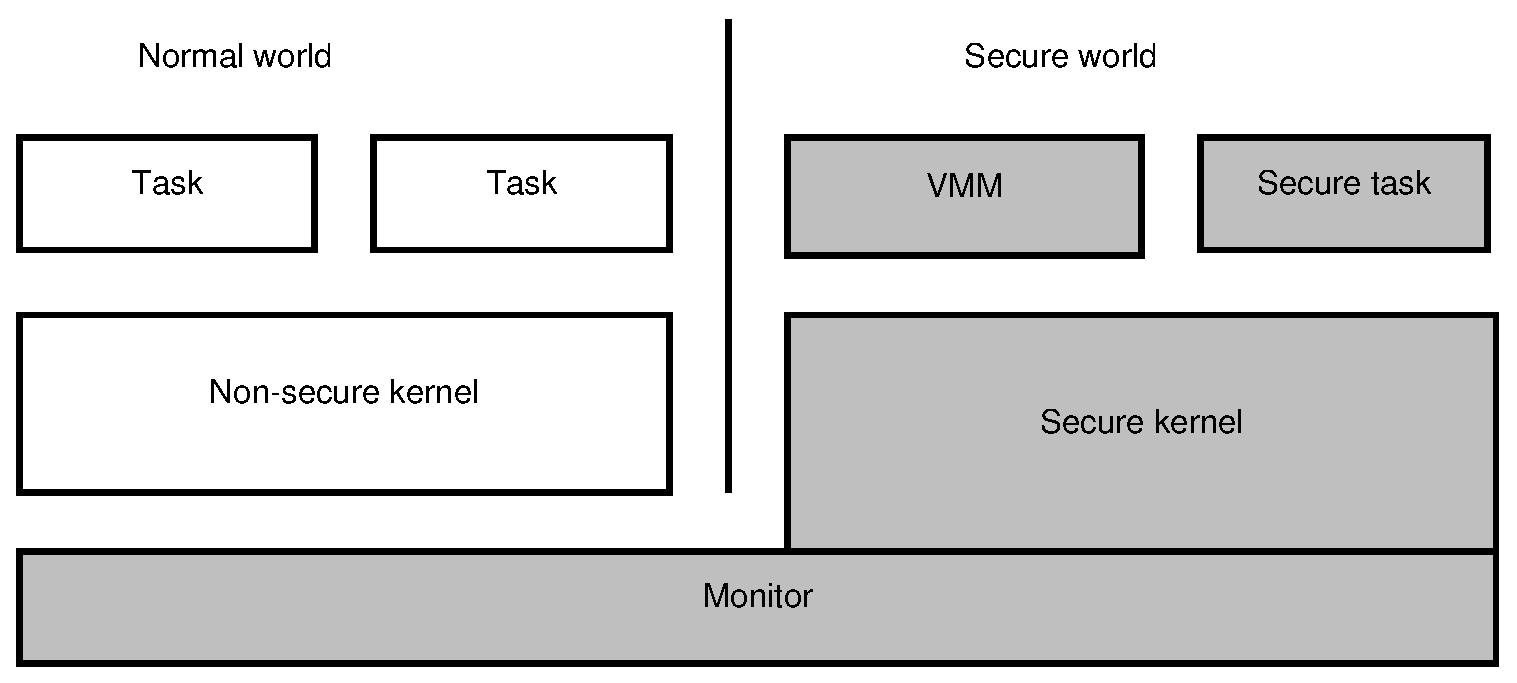
\includegraphics[width=0.9\linewidth]{./software_model}
\caption{}
\label{fig:software_model}
\end{figure}

% % % % % % % % % % % % % % % % % % % % % % % % % % % % % % % % % % % % % % % % %
\section{Последовательность загрузки}

\begin{itemize}
\item процессор стартует с secure world
\item загружается secure OS
\item запускается, к примеру, какой-нибудь user-space vmm
\item он выделяет регион в памяти, настраивает доступ к нему из normal, мапит себе его
\item загружет в выделенный регион образ non-secure OS
\item далее вызывает код монитора
\item монитор делает что-то вроде переключения контекста
\item монитор сохраняет состояние secure world (регистры и прочее)
\item загружает состояние normal world (оно хранится в спец структуре)
\item переключает NS бит
\item и передает управление на точку входа normal OS
\end{itemize}
% % % % % % % % % % % % % % % % % % % % % % % % % % % % % % % % % % % % % % % % %
\section{Регистры сопроцессора}

\subsection{Secure configuration register} \label{sec:SCR}

\begin{verbatim}
MRC p15, 0, <Rd>, c1, c1, 0
MCR p15, 0, <Rd>, c1, c1, 0
\end{verbatim}

Данный регистр управляет:
\begin{itemize}
\item NS битом
\item То, в каком режиме обрабатываются исключения
\item Возможностью модификации битов A и I в регистре CPSR когда процессор находится 
в normal world
\end{itemize}

\begin{tabular}{lll}
\hline \rule[-2ex]{0pt}{5.5ex} \bf\No\ бита & \bf Название & \bf Описание \\ 
\hline \rule[-2ex]{0pt}{5.5ex} 0 & NS & Определяет в каком мире сейчас находится \\
										& & процессор\\ 
										& & 0 = secure world\\
										& & 1 = normal world\\
\hline \rule[-2ex]{0pt}{5.5ex} 1 & IRQ & Определяет как происходит обработка IRQ  \\ 
\hline \rule[-2ex]{0pt}{5.5ex} 2 & FIQ & Определяет как происходит обработка FIQ \\ 
\hline \rule[-2ex]{0pt}{5.5ex} 3 & EA &  Определяет как происходит обработка \\ 
										& & external aborts\\ 
\hline \rule[-2ex]{0pt}{5.5ex} 4 & FW &  Установленный в 1 разрешает модификацию \\
										& & бита F регистра CPSR\\ 
\hline \rule[-2ex]{0pt}{5.5ex} 5 & AW &  Установленный в 1 разрешает модификацию \\
										& & бита A регистра CPSR\\ 
\hline 
\end{tabular} 

Этот регистр доступен для чтения и записи, но только из secure world.
За более подробной информацией обращайтесь к разделу 3.2.28 ARM Cortex-A8 Technical
Reference Manual.

\subsection{Monitor vector base address register} \label{MVBAR}

\begin{verbatim}
MRC p15, 0, <Rd>, c12, c0, 1
MCR p15, 0, <Rd>, c12, c0, 1
\end{verbatim}

Данный регистр предназначен для хранения базового адреса вектора монитора. Он доступен
на чтение и записть из привилегированного режима secure world.


% % % % % % % % % % % % % % % % % % % % % % % % % % % % % % % % % % % % % % % % %
\section{MMU}

Регистры MMU, такие как TTBR0, TTBR1 и TTCR являются banked между мирами, т.е. 
в каждом мире есть своя копия этих регистров, что позволяет иметь в каждом мире
свои таблицы трансляции адресов.


% % % % % % % % % % % % % % % % % % % % % % % % % % % % % % % % % % % % % % % % %
\section{L4re API для работы с TrustZone}

Для работы с TrustZone в l4re предусмотрен объект VM.
Создать который можно следуюшим образом:

\begin{verbatim}
#include <l4/sys/vm>

L4::Cap<L4::Vm> vm;
l4_msgtag_t msg = L4Re::Env::env()->factory()->create_vm(vm);
\end{verbatim}

Запуск non-sesure OS осуществляется с помощью метода run:
\begin{verbatim}
vm->run(_state_fpage, &_label);
\end{verbatim}
где state\_fpage --- flex page содержащая адрес структуры, где храниться
состояни normal world. Ниже представлено содержимой этой структуры (она описана
в файле pkg/l4sys/include/ARCH-arm/vm.h):
\begin{verbatim}
struct l4_vm_state
{
  l4_umword_t r[13]; // r0 - r12

  l4_umword_t sp_usr;
  l4_umword_t lr_usr;

  l4_umword_t sp_irq;
  l4_umword_t lr_irq;
  l4_umword_t spsr_irq;

  l4_umword_t r_fiq[5]; // r8 - r12
  l4_umword_t sp_fiq;
  l4_umword_t lr_fiq;
  l4_umword_t spsr_fiq;

  l4_umword_t sp_abt;
  l4_umword_t lr_abt;
  l4_umword_t spsr_abt;

  l4_umword_t sp_und;
  l4_umword_t lr_und;
  l4_umword_t spsr_und;

  l4_umword_t sp_svc;
  l4_umword_t lr_svc;
  l4_umword_t spsr_svc;

  l4_umword_t pc;
  l4_umword_t cpsr;

  l4_umword_t exit_reason;
};
\end{verbatim}

Возврат из метода run происходит после вызова smc из non-secure OS, после чего можно
снова вызвать run и non-secure OS продолжит свое иполнение.

Перед первым запуском vm не обходимо установить начальный значения регистров pc и 
cpsr. Например:
\begin{verbatim}
l4_vm_state state;

state->pc = 0x81000000;
state->cpsr = 0x13;
\end{verbatim}

Простой пример VMM работающего в l4re можно посмотреть \href{https://github.com/decaprox/l4re-snapshot/blob/020a76e63290159bcedc18b060108eab951be27e/src/l4/pkg/tz-vmm/server/src/main.cc}{здесь}.

\end{document}
